% !TEX root = ../CSS-OS.tex

\chapter{模拟程序的设计}

\MT{本章内容主要是程序整体框架的设计。主要目标是设计出一套便于实现和维护的架构,同时要易于进行扩展。}

\section{需求分析}


\section{交互接口}

\section{程序的主要逻辑——流程图}

\MT{目前版本的程序的逻辑(流程图)还处于比较初级的状态,所能考虑的情况还是比较少的,且有些条件的实现还比较的粗糙。}

\begin{figure}
\centering
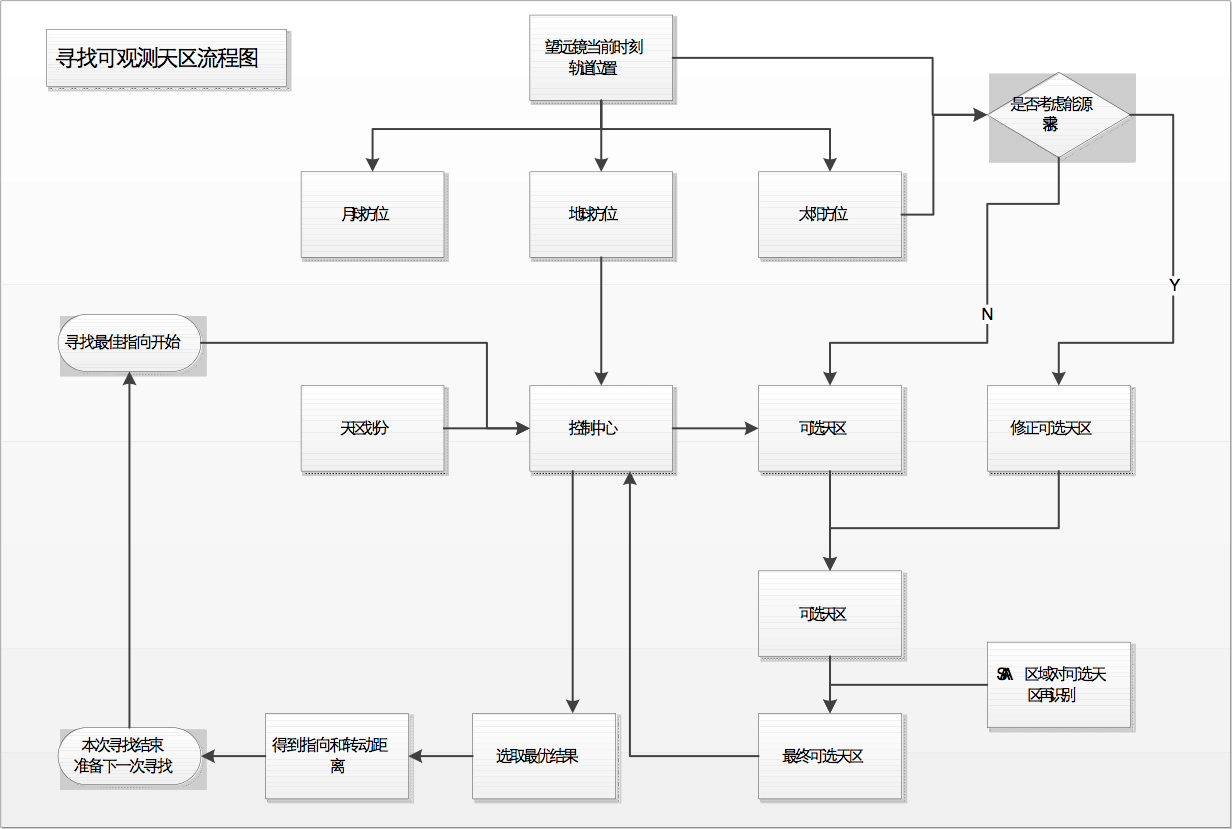
\includegraphics[width=\textwidth]{figs/flowchart.png}
\caption{寻找可观测天区流程图}
\label{fig:flow}
\end{figure}

\section{程序各模块的功能以及测试}
